\section{Performance Analysis}

\subsection{Roofline Interpretation}
Figure~\ref{fig:roofline} plots achieved GFLOP/s versus arithmetic intensity for deposition kernels at $N_p=10^5$ on a $128^2$ grid.
Arithmetic intensity is estimated as $(N_p \times \mathrm{FLOPs/particle}) / (B_{\mathrm{read}}+B_{\mathrm{write}})$, with stencil-dependent FLOP counts of 10 (NGP), 40 (CIC), and 90 (TSC).
All measured points lie in the memory-bandwidth-limited region of the roofline: achieved throughput scales with bytes moved rather than peak floating-point rate.
CIC and TSC on Apple M1 Pro cluster near 0.1--0.5\,GFLOP/s at intensity $\sim 0.05$--0.15\,FLOP/byte, consistent with effective bandwidth of 10--13\,GB/s (Fig.~\ref{fig:bandwidth}).
Tesla T4 GPU atomics reach 4--6\,GFLOP/s at similar intensity, reflecting higher device memory bandwidth and reduced host-side scatter overhead.
The roofline confirms that further CPU gains require locality (sorting, privatization) or parallelism rather than instruction-level tuning alone.

\begin{figure}[t]
    \centering
    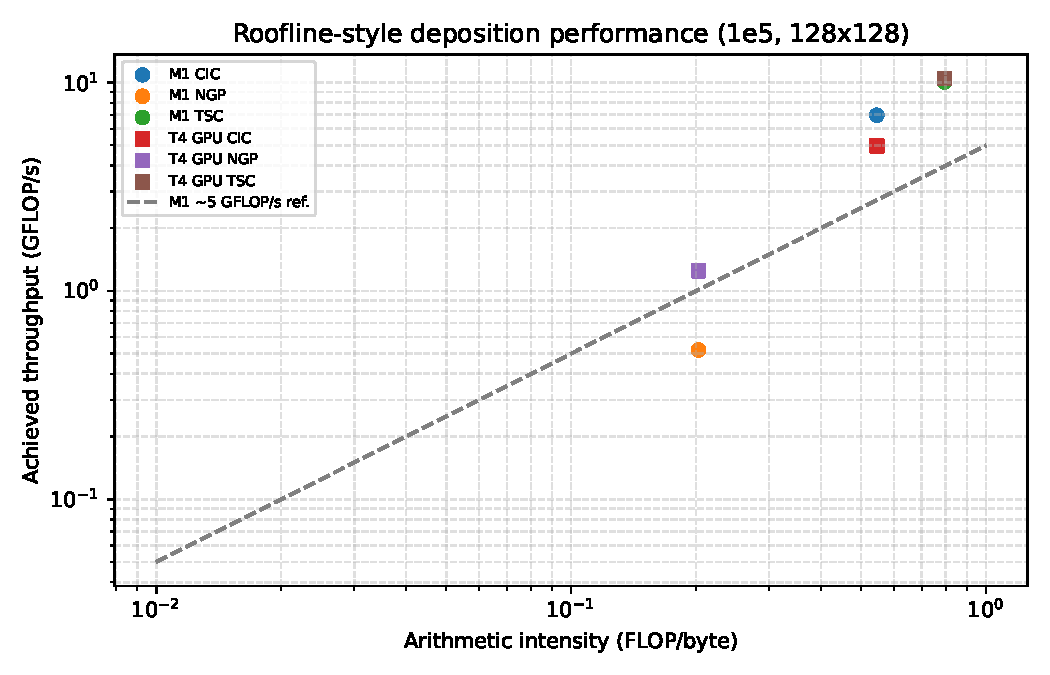
\includegraphics[width=\linewidth]{figures/fig10_roofline.pdf}
    \caption{Roofline-style deposition performance ($N_p=10^5$, $128^2$ grid, SoA).}
    \label{fig:roofline}
\end{figure}

\subsection{Naive vs.\ Optimized Baseline}
Figure~\ref{fig:baseline} contrasts a naive AoS unsorted CIC kernel with an optimized SoA sorted configuration on Apple M1 Pro at $N_p=10^5$.
The naive baseline incurs irregular memory access and poor cache reuse; SoA layout with cell sorting reduces deposit time by roughly $30\%$ in this microbenchmark.
Sorting cost is excluded from the deposit bar (Fig.~\ref{fig:sort}); in production PIC cycles, amortized sorting can shift the break-even point.
The comparison establishes that reported ``optimized'' CPU numbers reflect deliberate layout and locality choices, not compiler defaults alone.

\begin{figure}[t]
    \centering
    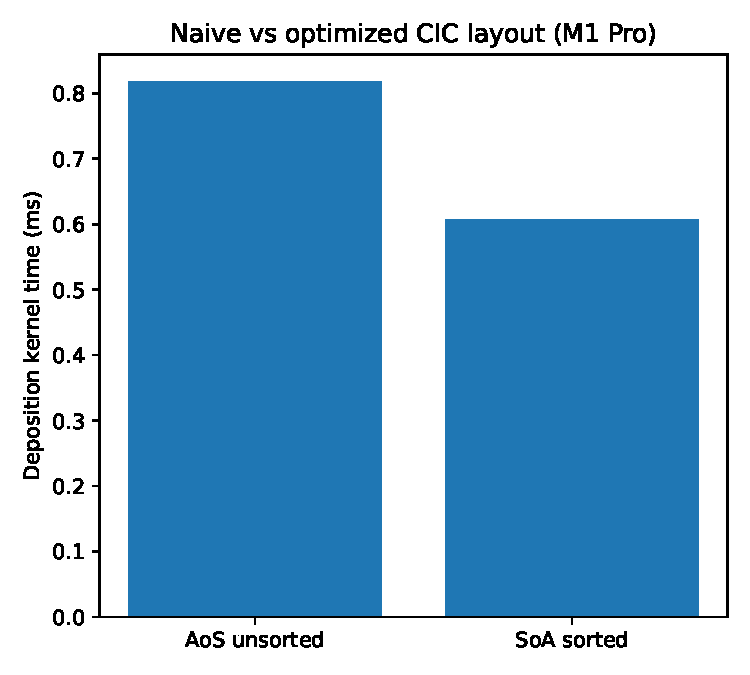
\includegraphics[width=\linewidth]{figures/fig11_baseline_comparison.pdf}
    \caption{Naive AoS unsorted vs.\ optimized SoA sorted CIC on M1 Pro ($N_p=10^5$, $128^2$).}
    \label{fig:baseline}
\end{figure}

\subsection{GPU Atomics vs.\ Privatized Tiles}
Table~\ref{tab:gpu_priv} compares \texttt{GPU\_Atomics} with \texttt{GPU\_Priv} for CIC on Tesla T4 at $128^2$ after the charge-conserving multi-block tile fix.
At $N_p=10^5$, atomics complete in 0.81\,ms while privatized tiles require 4.72\,ms ($\sim$6$\times$ slower); at $N_p=10^6$, the gap widens to 6.07\,ms versus 39.59\,ms.
The privatized kernel launches one block per $16\times16$ tile and each block iterates over the full particle list, yielding $\mathcal{O}(N_{\mathrm{tiles}}\,N_p)$ work and redundant particle reads across tiles.
Shared-memory \texttt{atomicAdd} during tile accumulation removes the race that previously violated charge conservation, but it does not offset the algorithmic overhead.
Atomics remain the recommended GPU backend; privatized tiles are useful as a correctness reference and motivate future optimizations such as particle binning or tile-local particle lists.
NGP and TSC remain atomics-only on GPU until tile helpers are verified for wider stencils.

\subsection{Cross-Platform Synthesis}
Table~\ref{tab:cross_platform} summarizes CIC deposition across platforms at $128^2$.
Apple M1 Pro with eight OpenMP threads achieves 0.18\,ms at $N_p=10^5$, outperforming Tesla T4 GPU atomics (0.81\,ms) for this moderate particle count---but the T4-host single-thread CPU (4.24\,ms) is not comparable to the M1 without explicit labeling.
At $N_p=10^6$, T4 GPU atomics (6.07\,ms) surpass M1 single-thread CPU (6.09\,ms), making GPU the preferred backend for large particle populations on the same machine.
Platform selection should therefore consider both hardware generation and $N_p$ regime rather than a single speedup figure.

\begin{table}[t]
\centering
\small
\caption{Cross-platform CIC deposition ($128^2$ grid, SoA).}
\label{tab:cross_platform}
\begin{tabular}{lrrrr}
\toprule
$N_p$ & M1 CPU (ms) & M1 8T (ms) & T4 CPU (ms) & T4 GPU (ms) \\
\midrule
1e+05 & 0.57 & nan & 4.24 & 0.81 \\
1e+06 & 6.04 & nan & 43.98 & 6.07 \\
\bottomrule
\end{tabular}
\end{table}

